
%% CLASS MANUAL FOUND IN http://blog.poormansmath.net/latex-class-for-lecture-notes/ %%
%% CLASS AUTHOR Stefano Maggiolo %%
\documentclass[english,course]{Notes}

\title{MATHS 2P : Graphs \& Networks}
\subject{Discrete Mathematics}
\author{Joao Almeida-Domingues}
\email{2334590D@student.gla.ac.uk}
\speaker{Professor Tara Brendle}
\date{25}{09}{2019}
\dateend{04}{12}{2019}
\place{University of Glasgow}

 %%%%% GENERAL MATHEMATICAL NOTATION SHORTCUTS %%%%%
 
\newcommand{\n}{\mathbb{N}}
\newcommand{\z}{\mathbb{Z}}
\newcommand{\q}{\mathbb{Q}}
\newcommand{\cx}{\mathbb{C}}
\newcommand{\real}{\mathbb{R}}
\newcommand{\field}{\mathbb{F}}
\newcommand{\ita}[1]{\textit{#1}}
\newcommand{\oneton}{\{1,2,3,...,n\}}
\newcommand\ef{\ita{f} }
\newcommand\inv[1]{#1^{-1}}
\newcommand\setb[1]{\{#1\}}
\newcommand\en{\ita{n }}
\renewcommand\qedsymbol{QED} %QED instead of square
\newcommand\placehold[1]{\begin{center}\includegraphics[width=#1\textwidth]{example-image-a}\end{center}}


%%%%%%%%%%%%%%%%PACKAGES%%%%%%%%%%%%%%%%%%%%%%%%%%%%%
%\usepackage{lipsum}  
\usepackage{todo}
\usepackage{amsmath,amsthm,amssymb,graphicx,mathtools,tikz} %maths
\usepackage{hyperref}
%\hypersetup{param1,param2,...} %overrides hyperreff package options setup in class
\usepackage{framed,color,fancybox} %layout
\usepackage{cleveref}
\usepackage{algorithm2e}
\renewcommand{\abstractname}{\vspace{2\baselineskip}} %hack to remove abstract

% framed :  \begin{shaded,frame,snugshade or leftbar} \definecolor{shadecolor}{rgb}{XYZ} to change color
%fancybox: \shadowbox,ovalbox or doublebox
%\extra for Extra content layout box
%%%%%%%%%%%%%%%%%%%%%%%%%%%

%%%CLASS SHORTCUTS%%%%
%\lecture{day}{month}{year} for margin note 
%\begin{theorem} sdfsdf\end{theorem}  --> \theorem
%\begin{proposition} dfsdfs\end{proposition} --> \prop
%\begin{lemma} dsfsd \end{lemma} --> \lem
%\begin{corollary} f ffew \end{corollary}
%\begin{definition} fwewef w \end{definition} --> \defn
%\begin{example} feww e\end{example} --> \ex
%\begin{exercise} wefwe \end{exercise}
%\begin{remark} wef we \end{remark} --> \rem
%\begin{fact} wefe \end{fact}
%\begin{problem} wef ew \end{problem}
%\begin{conjecture} ewfew \end{conjecture}
%\begin{claim} few w \end{claim}
%\begin{notation} fewf \end{notation} --> \nota
%\mymarginpar for scriptsize margin
% bold vectors --> \vc
% Placeholder figure -> \placeholder
\begin{document}

\newpage
\vspace*{\fill}
\begin{abstract}
\par{These lecture notes were collated by me from a mixture of sources , the two main sources being the lecture notes provided by the lecturer and the content presented in-lecture. All other referenced material (if used) can be found in the \ita{Bibliography} and \ita{References} sections.}
\par{The primary goal of these notes is to function as a succinct but comprehensive revision aid, hence if you came by them via a search engine , please note that they're not intended to be a reflection of the quality of the materials referenced or the content lectured.}
\par{Lastly, with regards to formatting, the pdf doc was typeset in \LaTeX , using a modified version of Stefano Maggiolo's \href{http://blog.poormansmath.net/latex-class-for-lecture-notes/}{\underline{\textcolor{blue}{class}}}}
\end{abstract}
\vspace*{\fill}
\newpage
%%%%%%%%%%%%%%%%%%%%%%%%%%%%%%%%%%%%%%%%%%%%%%%%%%%%%%%%%%%%%%%%%%
\section{Fundamentals}
\lecture{25}{09}{2019}
\subsection{Graphs}

\par{A graph $G$ is a pair $(V,E)$, where $V$ is any finite set, and $E$ is a set whose elements are pairs of elements of $V$. We call the elements of $V$ the \ita{vertices}*\mymarginpar{* often also referred as nodes} of $G$ and those of $E$ its \ita{edges}. e.g. $G=\set{\set{a,b,c} , \set{ab,ac}}$}

\defn{Adjacent Vertices}{are vertices connected directly through an edge. Formally, if  $e = \set{u,v} \in E$ , then $u , v$ are adjacent}

\rem{Also referred to as \ita{neighbours}}

\defn{Incident Edges}{are edges which share a vertex. We say that they are \ita{``incident to v''}}

\lecture{27}{09}{19}
\subsubsection{Representing Graphs}

\begin{enumerate}
\item[] Pictorially \mymarginpar{Note that the representation need not be unique}
	\placehold{0.4}
	
\item[] Adjacency Matrix
 
 \mymarginpar{Note that this definition only holds for simple graphs, i.e without loops. But , it is easily generalised if the binary requirement is dropped} 
 \defn{Adjacency Matrix}{ is the $ n \times n$ binary matrix , where $n = |V|$ and $a_{ij} =1 \iff e = \set{u,v} \in E$ ; i.e iff $u , v$ are adjacent }
 
 $$ A= \left(\begin{matrix}0&1&1&1\\1&0&1&0\\1&1&0&1\\1&0&1&0\end{matrix}\right) $$
 
 \rem{In this course, we'll only deal with \ita{simple}, \ita{undirected} graphs. Note that AMs of this type have the nice property of being symmetric (see 2B notes for properties)}
\end{enumerate}

\subsubsection{Subgraphs}

\defn{Subgraphs}{ are graphs obtained by deleting edges and/or edges of another graph}

\defn{Induced Subgraph}{ is a graph formed by deleting only nodes and their incident edges. Formally: Let $W \subset V$, then the induced subgraph of G is given by $G[W] = \set{W , \set{\set{xy} | xy \in G }}$. We say that \ita{``G is induced by W''} }


\example{ 

$$ G(V) = \set{ \set{a,b,c} , \set{ab, ac}} \text{ and } U = \set{c}  \text{ then } G[U] = \set{\set{a,b,\cancel{c}} ,\set{ab,\cancel{ac}}}$$}

\defn{Spanning Subgraph}{ similar to the induced, but edges are deleted instead}

\lecture{2}{10}{19}
\subsection{Graph Properties}

\defn{Walk}{from $u$ to $v$ is a sequence of vertices $w1, \dots ,wp$ (for some natural number $p \geq 2$), with $w_{1} = u$ and $w_{p} = v$, such that $w_{i}w_{i+1}$ is an edge for every $1 \leq i \leq p - 1$\label{1:walk}}

\par{Informally, a walk is just a sequence of vertices, where each subsequent vertex added to the sequence forms an edge with the preceding one}

\defn{Trail}{a walk with distinct edges}

\defn{Path}{a walk with distinct vertices}

\rem{In general, every walk  between two vertices contains a path \todo*{Remove commented out cits}}%\cite{Diestel}} 

\example{For a graph $P(\set{a,b,c,d,e,f} , \set{ab,ac,ad,bc,bd,cd,de,ef,}$) , ~\todo*{Add pictorial representation}

\begin{itemize}
\item[]\textbf{Walk: } $W = \set{abcdeacd}$ 
\item[] \textbf{Trail :} $T = \set{abcdea} = W \setminus \set{cd}_{2} $ 
\item[] \textbf{Path: } $P = \set{abcde} = W \setminus \set{acd}_{2}$ 
\mymarginpar{where $\set{x}_{2}$ is improper notation for the repeated instances of x in a set}
\end{itemize}
}
\prop{Number of Paths }{For a graph with $n$ vertices, there are $(n-1)^{n}$ paths}~\todo*{proof paths}
\defn{Connected}{A graph $G = (V, E) $ is connected if, for every two distinct vertices $u , v \in V$, there is a path in $G$ from $u$ to $v$}

\rem{A single vertex graph is connected. Since it has not distinct vertices, we say that the definition holds \ita{vacuously}}

\defn{Connected Component}{$H$ is a connected 
component of $G$ if $H$ is a connected induced subgraph of $G$ and, for
any subgraph $H'$ of $G$ such that $V(H) \subset V(H'), H'$ is not connected}

\rem{The vertex sets of distinct connected components are necessarily disjoint}

\placehold{0.4}

\defn{Vertex Degree}{$d(v) = |E(v)|$ , i.e. it is the size of the set of all edges connected to $v$}

\defn{Minimum Degree}{$\min _{v \in V(G)} d(v)$ , i.e. a graph's minimum degree is equal to the lowest degree of its vertices} \mymarginpar{The converse is true of the maximum}

\subsection{Isomorphisms}

\defn{Isomorphism}{from $G_{1} = (V_{1}, E_{1})$ to $G_{2} = (V_{2}, E_{2})$ is a
bijection $f : V_{1} \rightarrow V_{2}$ such that, for every $u, v \in V_{1}, f(u) f(v) \in E_{2}
\equiv uv \in E_{1}$}

\rem{Specifically, we can consider $f$ to be a process whereby one \ita{relabels} the vertices}

\placehold{0.5}

\todo{methods to determine isomorphism}
%%%%%%%%%%%%%%%%%%%%%%%%%%%%%%%%%%%%%%%%%%%%%%%%%%%%%%%%%%%%%%%%%%%%%%%%%%%%%%%%%%%%%%%%
\section{Special Graphs}

\defn{Complete Graphs}{Every pair of distinct vertices forms an edge}

\notation{$K_{n}$ , for a graph with $n$ vertices}

\prop{Number of Edges}{ \ $K_{n}$ has $\frac{1}{2}n(n-1)$ edges}~\todo{proof \#edges}

\defn{Paths}{a path on n vertices is a graph that is isomorphic to the graph $(V, E)$ where $V = \set{v_{1}, \dots, v_{n}}$ and $E = \set{v_{i}v_{i+1}}: 1 \leq i \leq n - 1$}
\notation{$P_{n}$}

\rem{$P_{n} $ has $n-1$ edges}

\defn{Cycle}{a cycle on $n$ vertices is a graph that is isomorphic to the graph $(V, E)$ where $V=\set{v_{1}, \ldots, v_{n}} \text{ and } E=\set{v_{i} v_{i+1}}: 1 \leq i \leq n-1 \cup \set{v_{n} v_{1}}$. i.e, it's a path with the end vertices connected}

\notation{$C_{n}$}
%%%%%%%%%%%%%%%%%%%%%%%%%%%%%%%%%%%%%%%%%%%%%%%%%%%%%%%%%%%%%%%%%%
\section{Trees}

\defn{Forest}{an \ita{acyclic} graph, i.e. without cycles}

\defn{Tree}{connected acyclic graph}

\defn{Leaf}{vertex of degree 1}

\placehold{0.5} 

\todo{Take fig.1 from lectures and connect the adjacent endpoints of all trees do contrast with forest}

\subsection{Basic Properties}

\prop{Leafs }{Every tree as at least one leaf}

\prop{Number of Edges }{$T_{n} \implies |E(T)| = n-1$}

\prop{Connected Graph }{Every connected graph with $n$ vertices and $n-1$ edges is a Tree}

\prop{Forests }{For a forest $F_{n}$ with $c$ connected components , $|E(T)| = n-c$}

\rem{Hence, note that a tree is just a special case of a forest, where $c=1$}

\subsection{Spanning Trees}

\defn{Spanning Tree}{Spanning subgraph which is not a tree}~\todo{Add example of sp.sub  is vs is not}

\placehold{0.5}

\prop{Necessity}{Every connected graph contains a spanning tree}

\begin{theorem}{Cayley's Formula : A complete graph with $n$ vertices has $n^{n-2}$ (labelled) spanning trees}~\label{2:caley}\end{theorem}

\par{It follows from \ref{2:caley} that , if we're interested in finding a \ita{minimum spanning tree} (a weighted sp.tree of minimum weight), an exhaustive search through all possible trees becomes a gruelling task very quickly. There are however two \ita{greedy} algorithms which help}

\subsection{Kruskal's Algorithm}

\par{For every edge not in the tree, add the one which has minimum weight and does not form a cycle. Stop when connected}

\begin{algorithm}[H]
\SetAlgoLined\KwData{this text}
\KwResult{how to write algorithm with \LaTeX2e }initialization\;
	\While{not at end of this document}{read current\;
		\eIf{understand}{go to next section\;
			current section becomes this one\;
		}{go back to the beginning of current section\;
		}
	}
\caption{How to write algorithms}
\end{algorithm}

\todo*{Add Kruskal's typesetting. Change label to header}



\theorem{Kruskal's }{will always output a M.S.T}

\proofs{\mymarginpar{Reproduction not examinable, merely analysis}}

\subsection{Prim's}

\par{Similar to Kruskal's but instead of looking for $min(E)$, we look for the smallest which adjacent to a node in the last iteration}
%%%%%%%%%%%%%%%%%%%%%%%%%%%%%%%%%%%%%%%%%%%%%%%%%%%%%%%%%%%%%%%%%%%%%%%%%%%%%%%%%%%%%%%%
\section{Proof Techniques}

%%%%%%%%%%%%%%%%%%%%%%%%%%%%%%%%%%%%%%%%%%%%%%%%%%%%%%%%%%%%%%%%%%
\section{Bipartite Graphs}

\defn{Bipartite Graph}{ The set of vertices can be partitioned into two, and every edge has one endpoint in each partition}

\rem{A graph is bipartite \ita{iff} every connected component is bipartite}

\todo{Write it in algo form}

\par{Check if bipartite : (1) pick a v in V , and add it to V1 . Set V2 to empty ; (2) While V1 U V2 != V , keep picking vertices which are not in V1 or V2, but are adjacent to V1 or V2; (3) If adjacent to V1 and not V2 add to V2 and vice versa (4) if adjacent to both then not bipartite}

\rem{For disconnected graphs, this would be repeated for each connected component}

\defn{Complete Bipartite}{ For $G(V,E)$ , where $V = V_{1} \cup V_{2}$ such that $E = \set{v_{1}v_{2} : v_{1} \in V_{1} , v_{2} \in V2}$ . Informally, it is a complete graph which is also bipartite}

\notation{$K_{p,q}$ , where $p,q = |V_{1}| , |V_{2}|$}


\par{Practical modelling applications will be all cases where one is not interested , or there's simple no connection between elements within the elements of a set. For example, matching patients with a certain disease to genetic anomalies in certain genes}

\subsection{Characterisation} 

\defn{Closed Walk}{Sequence of vertices $w_{1},\dots,w_{p}$ , such that $w_{i}w_{i+1}$ , for $p \geq 3$ and $1 \leq i \leq p-1$ and with $w_{1}w_{p}$ as an edge}

\rem{It is essentially a sort of cycle which allows for repeated vertices}

\placehold{0.5}
\todo{\url{https://slideplayer.com/slide/14901866/}}

\defn{Distance}{ between two vertices $u,v$ is the number of edges in the shortest path between $u$ and $v$}

\notation{$d(u,v)$}

\begin{theorem} G is bipartite \ita{iff} it contains no cycle of odd length as a subgraph \end{theorem}

\mymarginpar{expected to reproduce some part of}
\proofs{} 

\subsection{Matchings}

\defn{Matching}{set of independent edges , i.e. a set of edges from which no two have a common endpoint.}

\defn{Perfect Matching}{a matching that covers all the vertices, i.e. a bijection $f_{M} : V_{1} \to V_{2}$ where each $v \in V_{1}$ is mapped to the other endpoint of the edge in M that is incident with $v$}

\defn{Neighbourhood}{If $X$ is a set of vertices in $G$, then the neighbourhood of $X$ in $G$ is the set of all vertices in $G$ which have a neighbour in $X$}

\notation{$N_{G}(X)$}

\begin{theorem}
	\textbf{Hall's Marriage Theorem :} Let $G$ be a bipartite graph with bipartition $(U,W)$, where $|U| = |W| = p$. Then G contains a perfect matching \ita{iff} for all $U' \subseteq U$ , we have $|N_{G}(U')| \geq |U'|$
\end{theorem}

\rem{ every subset $U'$ of $U$ has sufficiently many adjacent vertices in $W$.}

\mymarginpar{Complex}
\proofs{ See lecture notes}

\example{}
\par{A common illustration of the theorem is in pairing couples. If in a group of $k$ people there's a total of $k-1$ options, then there can be no perfect matching. Say for example, that two people find the same and only that person acceptable, then one of them will be left unmatched. In this case the subset of people $U= \set{u_{1}, u_{2}}$ , while their matching set , their neighbourhood $ W=\set{w_{2}}$. We have then, $|U| = 2 \leq |W| = 1$}

\IfFileExists{hallExample.png}{}{\write18{wget https://cdn.mathpix.com/snip/images/bPNzKL84kHw9E1U8HWUzvQ8QmXQUO_sQvz3eXeIiTNE.original.fullsize.png -O hallExample.png}}

\begin{figure}[ht]
\centering
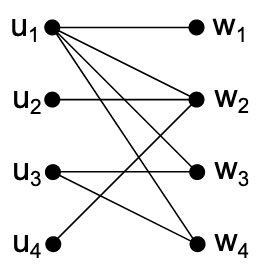
\includegraphics[width=0.3\textwidth]{hallExample.png}
\end{figure}



\section{Colouring}

\defn{Proper k-colouring}{$f : V(G) \to \set{1,\dots,k} $ such that $f(u) \neq f(v)$ , whenever $uv \in E(G)$ , i.e we assign \ita{``colours}'' to each vertex, using only $k$ colours, so that no two adjacent vertices have the same colour}

\par{This can be done trivially, by simply assigning a different colour to each vertex, however often colouring problems fall within the optimisation category, where we look to minimise the number of colours used}

\defn{Chromatic Number}{Smallest number $k$ such that $G$ is colourable}

\notation{$\chi(G)$}

\defn{Clique}{Complete subgraph}

\defn{Clique Number}{Largest  $t$ , such that $K_{t}$ is an induced subgraph of $G$, i.e. $|max(Clique(G))|$}

\rem{In other words, the subgraph formed by removing the least amount of vertices, so as to make G complete}

\notation{$\omega(G)$}

\subsection{Chromatic Number and Graph Properties}

\par{Finding the chromatic number of a graph is an np-hard problem, so in general we use certain techniques in order to find a lower bound}

\begin{enumerate}
\item If $H$ is a subgraph of $G$ and $\chi(H) \geq k$, then $\chi(G) \geq k$

\item $\chi(K_{n}) = n$
\end{enumerate}

\par{From this, we deduce that $\chi(G) \geq \omega(G)$} 

\defn{Independent Set}{For $U \subseteq V$ if no edge in $E$ has both endpoints in $U$}

\defn{Independence Number}{size of the largest independence set}

\notation{$\alpha(G)$}

\rem{Note that by definition, every partition in a bipartite graph is an independent set}

\par{Note then that

\begin{theorem}{For $|V(G)| = n$ , $\chi(G) \geq \frac{n}{\alpha(G)}$}\end{theorem}
\todo{proof lower bound chrom\&indp}
\mymarginpar{expected to reproduce some part of}
\proofs{}


\subsection{Greedy Algorithm}

\lemma{For $max(V(G)) = d$ , $\chi(G) \leq d + 1$}

\mymarginpar{Full reproduction expected}
\todo{lower bound chromatic}
\proof{}


\newpage

\todo*{BibTex : Diestel,Reinhard ; Graph Theory}

\todos

\end{document}

